\chapter{Development Process \& Contributing to MATSim \who{Horni, Rieser, Nagel}}
\label{ch:developmentprocess}
% ##################################################################################################################

\kai{Ich w�rde gerne ``Development process'' und ``Contributing to MATSim'' auftrennen.  Ersteres beschreibt Dinge wie core development, regression tests, etc.  Aber ``contributing to MATSim'' sollte sich auf die extension points konzentrieren.  Vielleicht zusammen mit dem vorhergehenden Kapitel.}

\hfill \textbf{Author:} Andreas Horni

\begin{center} 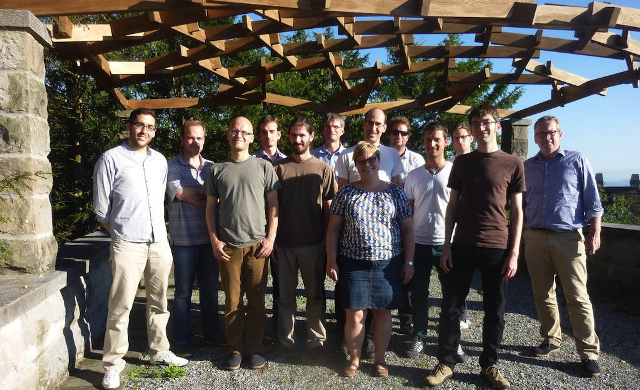
\includegraphics[width=0.5\textwidth, angle=0]{extending/figures/ConceptualMeetingVillaHatt.png} \end{center}

% ##################################################################################################################
This chapter describes how new functionality enters MATSim. It describes the MATSim community, development drivers and processes, and tools used for integration.

\ah{Vieles noch etwas zu implizit dargestellt! -> Aufz�hlungen einf�gen. Playgrounds! Testing! Verantwortlichkeiten!}

\ah{matsim-devel\@lists.sourceforge.net}

\ah{approx. number of playgrounds}

\ah{approx number of code lines /classes at the different locations (core, playgrounds, contributions etc.}

% ##################################################################################################################
\section{MATSim Community}
The core of the MATSim community are three research groups and a spin-off company, namely 
\begin{itemize}
\item the Transport Systems Planning and Transport Telematics group at the Institute for Land and Sea Transport Systems, Technische Universit�t Berlin, led by Prof. Dr. Kai Nagel,
\item the Transport Planning group at the Institute for Transport Planning and Systems (IVT), Swiss Federal Institute of Technology Zurich, led by Prof. Dr. Kay W. Axhausen, 
\item the recently founded Mobility and Transportation Planning group at the Future Cities Laboratory, based in Singapure and lead by Prof. Dr. Kay W. Axhausen, and 
\item senozon AG, based at Z�rich with a subsidiary in Germany, founded by former PhD and research students. 
\end{itemize}

As common in research the three university groups' composition changes frequently. Over the last decade around 20 people build the MATSim core, where the recently founded Singapore increases that number by another handful of persons. An overview of current and former MATSim contributors can be found at ....  

The core groups of MATSim are in close contact with other research groups using and extending MATSim. Toronto (Canada), Pretoria (South Africa), Karlsruhe and J�lich (both Germany) are examples. Additionally, there are the MATSim users, usually contributing to development by informing about their achievements for example in the MATSim user meeting, or also reporting back their needs or problems with the software, and sometimes bugs. Although MATSim is an open-source program provided by the GNU General Public License version 2.0 (GPLv2), there is not yet a large external developer group that contributes for the sake of hacking detached from an own direct application need. However, the MATSim community is open and interested in further contributors, which are mentored in the beginning \citep[][]{MATSIM-T-BecomingAContributor_Webpage_2014} to become familiar with the project and the coding conventions \citep[][]{MATSIM-T-CodingGuide_Webpage_2014}.

Picture \ref{fig:team} shows a snapshot of the participants of the first conceptual meeting representing a good mix of core group members but also associated researchers.
%
% ------------
\createfigure%
{Participants of the first MATSim conceptual meeting at Villa Hatt in Z�rich in 2012}%
{Participants of the first MATSim conceptual meeting at Villa Hatt in Z�rich in 2012}%
{\label{fig:team}}%
{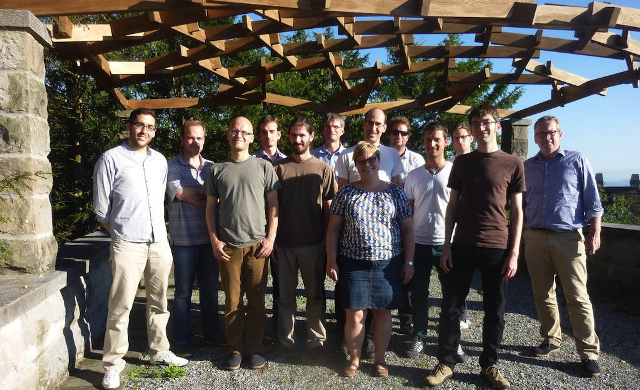
\includegraphics[width=0.99\textwidth, angle=0]{extending/figures/ConceptualMeetingVillaHatt.png}}%
{}
% ------------

% ##################################################################################################################
\section{Drivers and Organization of Development}
Main drivers of the MATSim development are the projects and dissertations accomplished by the MATSim core team. New features are developed as an answer to requirements of these dissertations and projects, where projects range from purely scientific ones (often sponsored by SNF) to projects for the administration (see e.g., Section \ref{sec:wu}), to projects where science and industry contribute equally (usually CTI-projects, see e.g., Section \ref{sec:ktizh}) and to purely industrial projects, which are managed by senozon AG in the majority of cases. A significant amount of innovation is also introduced by the collaboration with external researchers.

The continuous integration of innovation requires a substantial amount of management. Following organization has turned out to be productive. Derived from the types of MATSim use presented in Section \ref{sec:usingmatsim} different levels of code contribution exist. Users run MATSim as a tool with the configuration file. The MATSim API is targeted to be rather stable (\lstinline|package org.matsim.api.*|), thus, API-users do not necessarily need to be part of the MATSim repository. These two groups' contributions hence are indirect, i.e., usually limited to innovation in terms of content not code. Developers, however, contribute code directly;  they have at least their own playground in the MATSim project such that their code is considered by the refactorings. A relatively small circle of the developers is allowed to commit code to the MATSim core (\lstinline|package org.matsim.core.*|).

Systematic code integration is mainly performed by the Berlin group and by senozon AG. This includes continuous code review and integration upon request of the core community, but also comprehensive code refactorings to clean degenerated code. A huge refactoring greatly improving the code base structure and establishing the distinction between core, api and the remaining packages was undertaken by the Berlin group starting at the end of 2007 and ended in the beginning of 2009 before the first user meeting \ah{stimmt das so?}. Refactorings are documented in the MATSim issue tracker.

Code that is not directly related to the core functionality of MATSim, which is agent-behavior and transport simulation, goes to the MATSim contributions (\lstinline|package org.matsim.contrib.*|). Developers of contributions are usually MATSim developers.

The development process is supported by a standing MATSim committee discussing conceptual issues on a regular basis. Another element bringing in innovation but also organization are the annual meetings. Right from the beginnings, there has been a MATSim developer meeting focused on coding issues. Later, a user meeting giving insights into accomplished work by the community. Finally, a conceptual meeting has been added strictly dedicated to issues that go beyond pure software engineering. The developer and the conceptual meeting have shown to establish an effective road map, which has guided the development for the remainder of the year.

The internal development is organized by regular group meetings, in Z�rich for example by the ``MATSim group meeting'' and in Berlin by the ``jour fix''. 

Due to the heterogeneous character of the community and its individual research groups, with every developer engaged in his individual dissertation work, organizing the development in an agile and somewhat ad hoc manner has been regarded beneficial over adopting an established software project management method.

% ##################################################################################################################
\section{Development Tools and Techniques}
In the early days of MATSim, the code was programmed in C++. In 200x \ah{???}, however, the code was migrated to Java. Performance of Java and C++ had converged to a reasonable extent, such that the much higher developer friendliness of Java could be exploited. A fast access to the program is essential for MATSim as many api-developers have their background in fields such as transport planning or social sciences and not in computer science. 

Up to 2007, when MATSim was brought to Sourceforge \ah{REF}, MATSim was provided by a download website and svn repository hosted on a VSP server.

MATSim development makes use of a whole bunch of tools greatly leading to better software quality. Summarized and accessible from the MATSim website---with private access---a change log, an issue tracker, the javadoc, static code analyses performed by FindBugs and PMD, test code coverage analysis, copy paste analysis, code metrics, maven dependencies, the complete code linked by Xref, and the information about the nightly test results are provided. These nightly test results are generated by the MATSim build server based on Jenkins \ah{REF}. Furthermore, there is a MATSim benchmark available (http://www.matsim.org/docs/devguide/optimization).

Most MATSim developers use Eclipse \ah{REF} as an integrated development environment (IDE). The MATSim documentation is tailored to this IDE. Team development is based on Apache Subversion SVN \ah{REF}. A developer's mailing list is used for team communication besides others. External libraries dependencies are managed by Maven \ah{REF}. 

MATSim development furthermore greatly benefits from the possibility to run large-scale scenarios. Therefore, several servers with up to 512GB RAM and 40 CPU cores are available.  

\ah{etwas aus dem N�hk�stchen plaudern -> Issue-Tracker?}
\ah{modular approach}

% ##################################################################################################################
\section{Documentation, Dissemination and Support}
The main documentation can be found on the MATSim webpage \citep[][]{MATSIM-T-Docu_Webpage_2014}, where information is distinctly provided in a user's guide, an api-user's guide and developer's guide. Additionally, a handful of tutorials is available, with the ``Quickstart''-tutorial to get fast access to MATSim and the ``Learning MATSim in 8 Lessons''-tutorial, which is used for the user's meetings and hands-on tutorials in Berlin, Z�rich and occasionally elsewhere, also listed on that page. 

Code documentation in form of Javadoc can be found at \citet[][]{MATSIM-T-Javadoc_Webpage_2014}. 

For fast application of MATSim some small-scale example scenarios are provided in the code base (\lstinline|folder: src/test/resources/test/scenarios/|), where recently an extended version of the well-known benchmark scenario for the City of Sioux Falls has been added \citep[][]{ChakirovFourie_TechRep_FCL_2014}.

Further information is disseminated at the afore-described annual user meetings, and by the MATSim mailing lists (\lstinline|users@matsim.org| and \lstinline|api-users@matsim.org|) \citep[][]{MATSIM-T-Mailinglists_Webpage_2014}. Usually, also support is provided by the MATSim developers via these mailing lists. Particularly active in support are the Berlin group and senozon AG. A theoretical overview of all the components in MATSim is given by the numerous papers published in international journals and presented at worldwide conferences; an overview can be found at \citep[][]{MATSIM-T-Publications_Webpage_2014}. 

Apparently, the information on MATSim is quite extensive, however, getting a complete picture as a new MATSim user requires a substantial literature search effort. Reduction of this hassle is the goal of the book at hand.

% ##################################################################################################################
\section{Development in Recent Years}
\ah{Diskussion am Conceptual Meeting:

Classes and methods stabil seit Langem: 
auf was deutet das hin? Zu wenig Innovation oder Clean-Code? Steckt zuviel in den Playgrounds, Contribs oder ist das genau richtig?
Wurde Kernfunktionalit�t eingef�gt und daf�r weniger Zentrales (wie Evacuation) nach und nach in Contrib verschoben?

Der Drop Ende 2007, war das schon Core, Api Umstruktutierung oder war das die Entfernung von G. package?
}

\createfigure%
{Code development since 2005}%
{Code development since 2005}%
{\label{fig:codedev}}%
{%
  \createsubfigure%
  {...}%
  {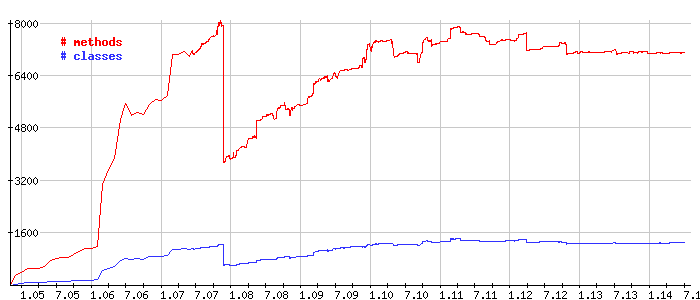
\includegraphics[width=0.95\textwidth,angle=0]{extending/figures/nof_classes.png}}%
  {\label{fig:codedev0}}%
  {}%
  \createsubfigure%
  {...}%
	{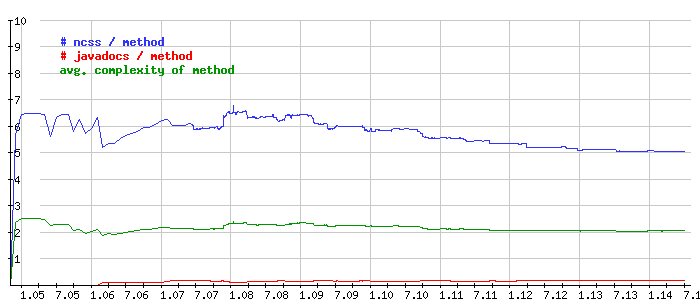
\includegraphics[width=0.95\textwidth,angle=0]{extending/figures/avg_method.png}}%
  {\label{fig:codedev1}}%
  {}%
}%
{}

\ah{
Meilensteine in den letzten Jahren?:

PT

DC (hehe)?

Modechoice?

Social networks?
}

% ##################################################################################################################



